% formal/stateless.tex
% mainfile: ../perfbook.tex
% SPDX-License-Identifier: CC-BY-SA-3.0

\section{Stateless Model Checkers}
\label{sec:formal:Stateless Model Checkers}
%
\epigraph{He's making a list, he's permuting it twice\dots}
	{\emph{with apologies to Haven Gillespie and J. Fred Coots}}

The SAT-solver approaches described in the previous section are quite
convenient and powerful, but the full tracking of all possible
executions, including state, can incur substantial overhead.
In fact, the memory and CPU-time overheads can sharply limit the size
of programs that can be feasibly verified, which raises the question
of whether less-exact approaches might find bugs in larger programs.

\begin{figure}
\centering
\resizebox{2.1in}{!}{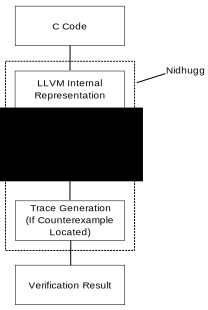
\includegraphics{formal/nidhugg}}
\caption{Nidhugg Processing Flow}
\label{fig:formal:Nidhugg Processing Flow}
\end{figure}

Although the jury is still out on this question, stateless model
checkers such as Nidhugg~\cite{CarlLeonardsson2014Nidhugg} have in
some cases handled larger programs~\cite{SMC-TreeRCU}, and with
similar ease of use, as illustrated by
Figure~\ref{fig:formal:Nidhugg Processing Flow}.
In addition, Nidhugg was more than an order of magnitude faster than
was \co{cbmc} for some Linux-kernel RCU verification scenarios.
Of course, Nidhugg's speed and scalability advantages are tied to
the fact that it does not handle data non-determinism, but this
was not a factor in these particular verification scenarios.

Nevertheless, as with \co{cbmc}, Nidhugg has not yet been able to
locate a bug that Linux-kernel RCU's maintainer was not already
aware of.
However, it was able to demonstrate that one historical bug in
Linux-kernel RCU was fixed by a different commit than the maintainer
thought, which gives some additional hope that stateless model checkers
like Nidhugg might someday be useful for finding concurrency bugs in
parallel code.
